\documentclass[aspectratio=169,10pt]{beamer}

\usepackage[T1]{fontenc}
\usepackage{lmodern}
\usepackage{amsmath,amssymb,bm}
\usepackage{booktabs}
\usepackage{graphicx}
\usepackage{siunitx}
\usepackage{tabularx}
\usepackage{array}
\usepackage{xcolor}
\usepackage{hyperref}
\usepackage{tikz}

\definecolor{navy}{HTML}{17365D}
\definecolor{slate}{HTML}{475866}
\definecolor{rulegray}{HTML}{CBD3DA}
\definecolor{recovery}{HTML}{A23B32}
\definecolor{softblue}{HTML}{E9F0F5}

\setbeamercolor{normal text}{fg=black,bg=white}
\setbeamercolor{frametitle}{fg=navy,bg=white}
\setbeamercolor{title}{fg=navy}
\setbeamercolor{structure}{fg=navy}
\setbeamercolor{block title}{fg=navy,bg=softblue}
\setbeamercolor{block body}{fg=black,bg=softblue!45}
\setbeamertemplate{navigation symbols}{}
\setbeamertemplate{itemize item}{\raise0.15ex\hbox{\scriptsize$\blacktriangleright$}}
\setbeamertemplate{frametitle}{%
  \vspace{0.22cm}\insertframetitle\par
  \vspace{0.06cm}{\color{rulegray}\rule{\textwidth}{0.45pt}}
}
\setbeamertemplate{footline}{%
  \hfill\raisebox{0.15cm}{\color{slate}\scriptsize\insertframenumber\hspace{0.35cm}}%
}
\setbeamersize{text margin left=0.62cm,text margin right=0.62cm}

\graphicspath{{neuronbench_evolve_pysr_supervisor_2026-08-28_latex_assets/}}
\newcommand{\source}[1]{%
  \begin{tikzpicture}[remember picture,overlay]
    \node[anchor=south west,text=slate,font=\tiny,text width=0.89\paperwidth]
      at ([xshift=0.62cm,yshift=0.13cm]current page.south west) {#1};
  \end{tikzpicture}%
}
\newcommand{\nrmse}{\operatorname{NRMSE}}
\newcommand{\phina}{\phi_{\mathrm{Na}}}
\newcommand{\phik}{\phi_{\mathrm{K}}}
\newcommand{\phiz}{\phi_{Z}}

\title{NeuronBench and \texttt{evolve\_pysr}}
\subtitle{Meta-evolving symbolic regression for mechanistic neuron dynamics}
\author{Grant update}
\date{28 August 2026}

\begin{document}

% 1
\begin{frame}[plain]
  \vspace{0.85cm}
  {\color{navy}\LARGE\bfseries NeuronBench and \texttt{evolve\_pysr}}\\[0.30cm]
  {\large Meta-evolving symbolic regression for mechanistic neuron dynamics}\\[0.72cm]

  \begin{minipage}{0.86\textwidth}
  \large
  \begin{itemize}
    \item Adapt six generalized Hodgkin--Huxley ``mystery neurons'' into exact, fully observable symbolic-regression problems.
    \item Evolve PySR mutation, survival, selection, and loss operators on subsets of neuron worlds, then evaluate transfer to held-out worlds.
    \item Newest ``uninformative prompt'' run (708907): \textbf{23/25 strict numerical recoveries}, plus two near-exact fits and no misses.
  \end{itemize}
  \end{minipage}

  \vfill
  {\color{slate}\small Primary references: Murphy, \emph{Model Discovery Agent}, arXiv:2608.09696v4; project runs 313196, 313195, 190177, and 708907.}
\end{frame}

% 2
\begin{frame}[t]{Original NeuronBench: active model discovery}
  \begin{columns}[T,onlytextwidth]
    \begin{column}{0.43\textwidth}
      \scriptsize
      Murphy's benchmark defines six ``mystery neurons'' using generalized Hodgkin--Huxley ODEs. Each has a novel membrane mechanism intended to be difficult to identify from textbook recall alone.

      \vspace{0.10cm}
      \begin{itemize}
        \item The agent chooses among nine current-clamp protocols.
        \item It observes voltage trajectories; gating state and mechanism are latent.
        \item It predicts six trajectory features under held-out interventions.
        \item MDA combines nested SMC$^3$, LLM model proposals, and Bayesian experiment design.
      \end{itemize}

    \end{column}
    \begin{column}{0.55\textwidth}
      \centering
      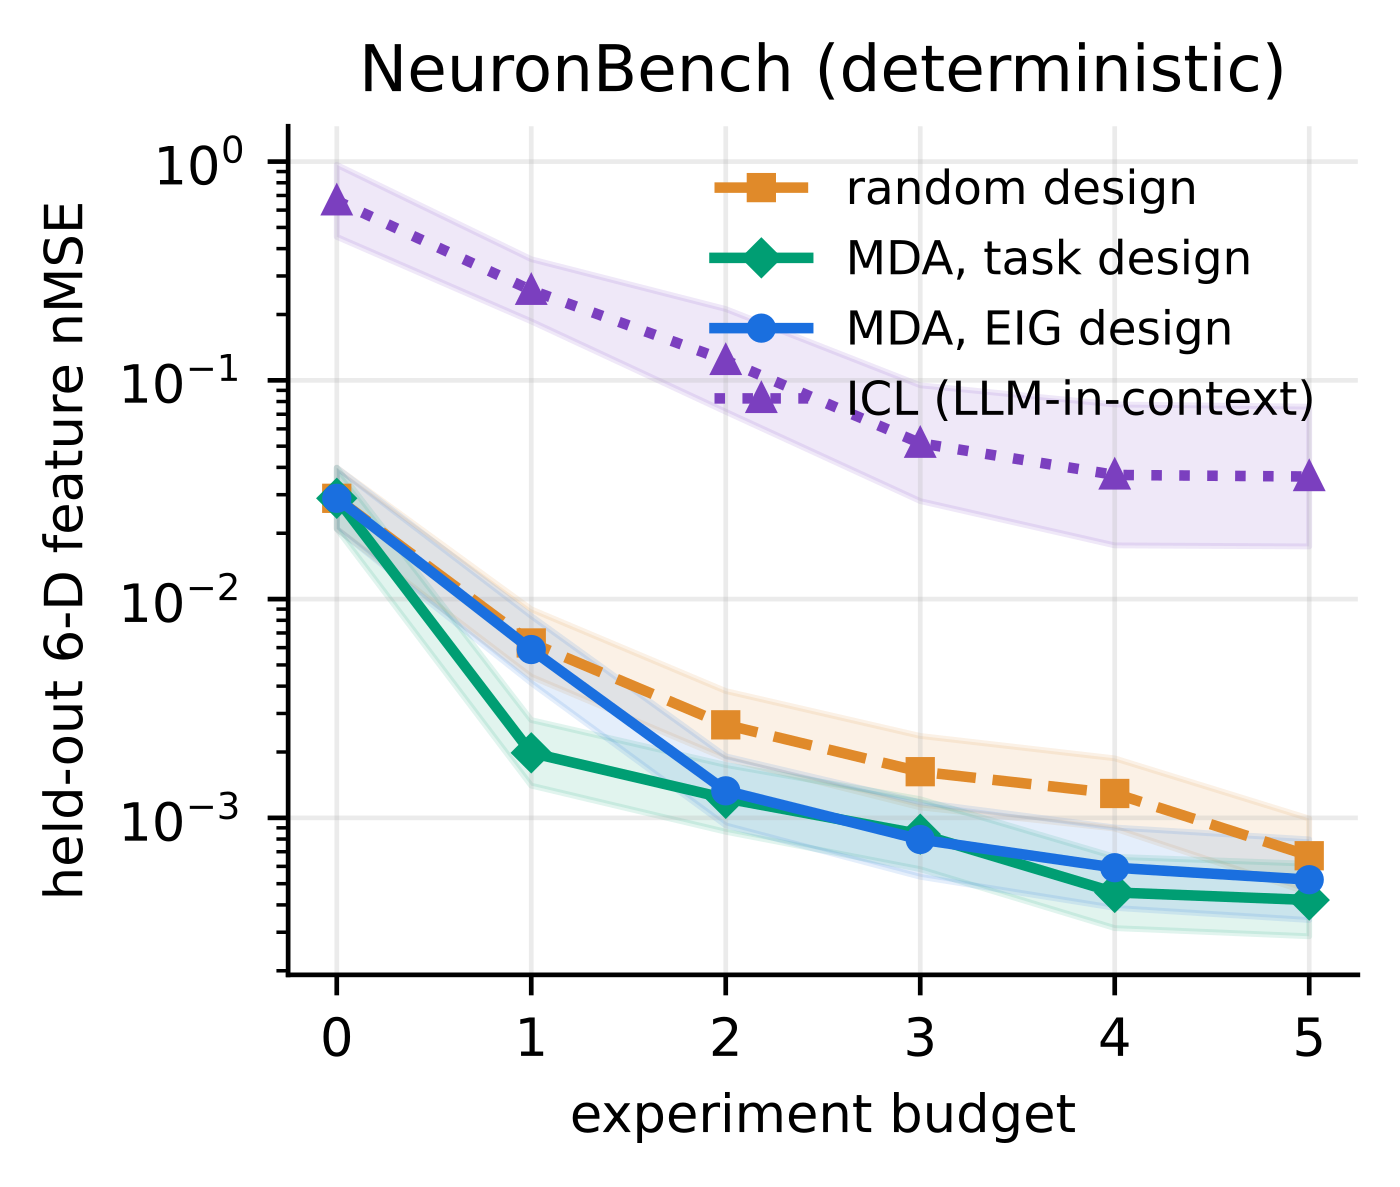
\includegraphics[width=0.88\linewidth]{murphy_fig4a.png}

      {\scriptsize Murphy Fig.~4(a): deterministic NeuronBench; mean $\pm$ SE.}
    \end{column}
  \end{columns}
  \source{Primary source: Kevin Murphy, \emph{Model Discovery Agent: LLM-assisted Bayesian experiment design for data-efficient discovery of mechanistic world models}, arXiv:2608.09696v4, Sec.~4.4 and Fig.~4(a).}
\end{frame}

% 3
\begin{frame}[t]{Our reduction: expose the state and recover the current balance}
  \begin{equation*}
    \dot V
    = I_{\mathrm{ext}}
    - \sum_c g_c\,\phi_c\,(V-E_c)
    - g_L(V-E_L).
  \end{equation*}

  \begin{columns}[T,onlytextwidth]
    \begin{column}{0.64\textwidth}
      \centering
      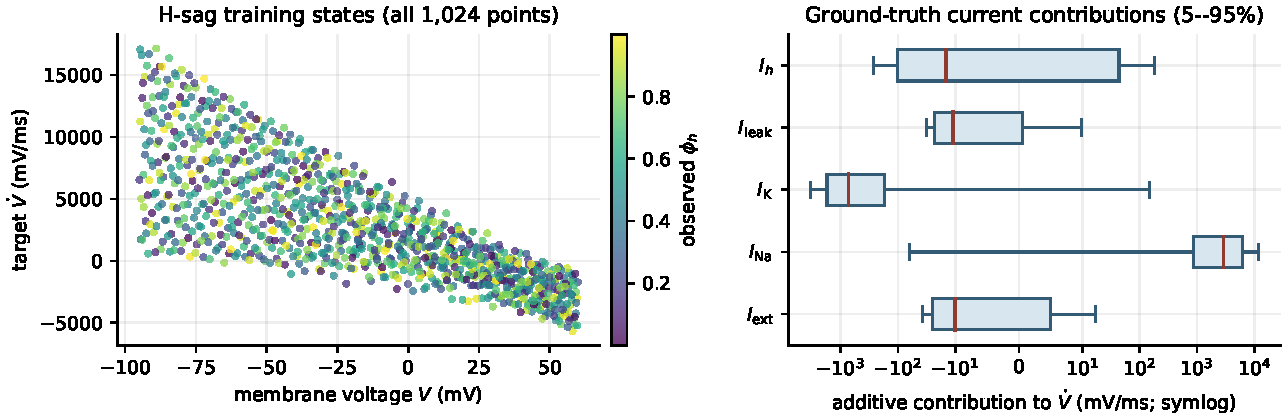
\includegraphics[width=0.96\linewidth]{raw_h_sag.pdf}
    \end{column}
    \begin{column}{0.34\textwidth}
      \scriptsize
      \textbf{What is changed}
      \begin{itemize}
        \item No active experiment selection.
        \item Observe $I_{\rm ext}$, $V$, and each composite open fraction $\phi_c$.
        \item Fit only the scalar vector field $\dot V$.
      \end{itemize}

      \textbf{Data protocol}
      \begin{itemize}
        \item 1,024 scrambled-Sobol training states.
        \item 16,384 held-out states.
        \item $V\in[-95,60]$ mV; $\phi_c\in[0,1]$.
        \item Analytic, noiseless targets.
      \end{itemize}
    \end{column}
  \end{columns}
  \source{Primary project data: \texttt{runs/neuronbench\_fully\_observable/data/h\_sag.npz}; generator and equation: \texttt{scripts/neuronbench\_fully\_observable.py}.}
\end{frame}

% 4
\begin{frame}[t]{Connection to the existing Sandia Hodgkin--Huxley project}
  \begin{equation*}
  C_m\dot V = I_{\rm ext}
  -g_{\rm Na}m^3h(V-E_{\rm Na})
  -g_{\rm K}n^4(V-E_{\rm K})
  -g_L(V-E_L).
  \end{equation*}
  \centering
  {\scriptsize The Sandia demonstration uses a canonical HH trajectory; NeuronBench retains the current law but tests six mechanisms on independent collocation states.}\par
  \vspace{0.04cm}
  \centering
  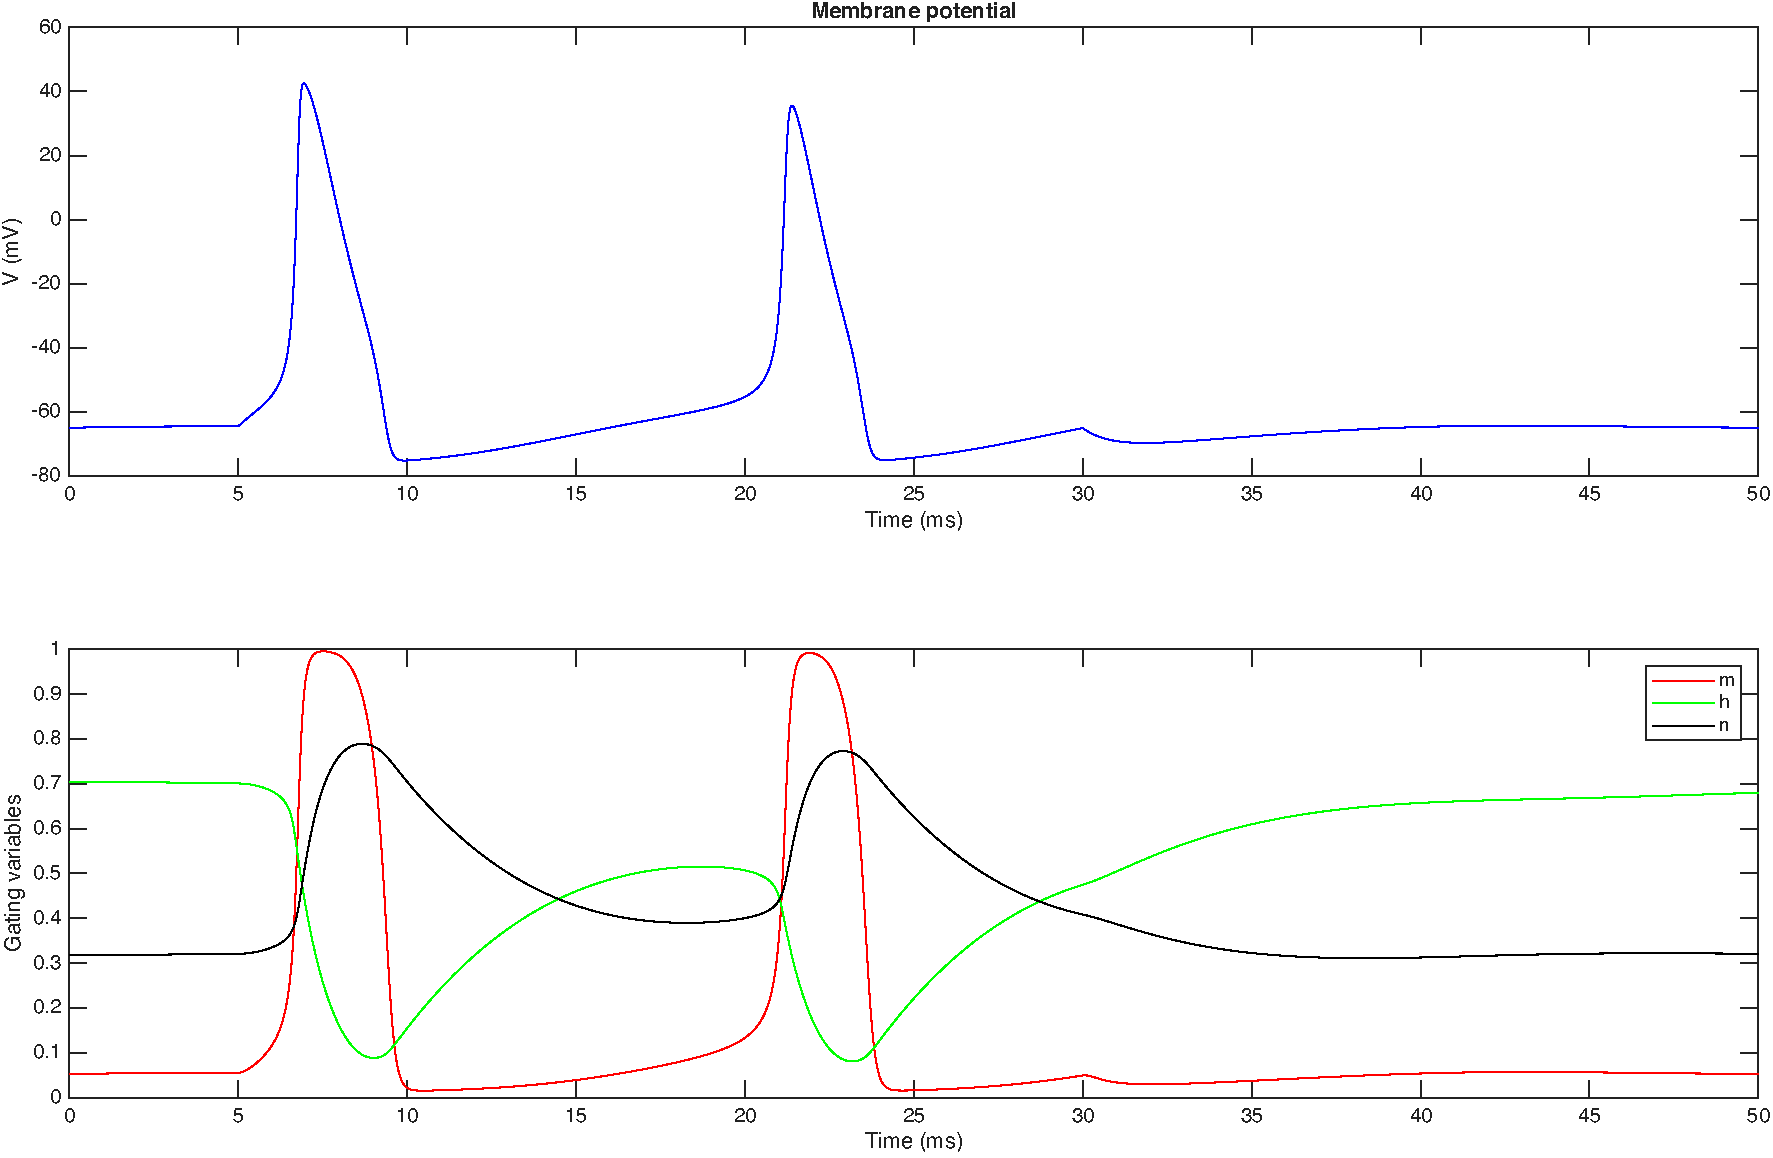
\includegraphics[width=0.88\linewidth,height=0.52\textheight,keepaspectratio]{sandia_hh_fig1.pdf}

  {\scriptsize Existing Sandia simulation: membrane potential and the $m,h,n$ gating variables.}
  \source{Primary local source: \texttt{/home/sca63/sandia\_spiking/Hodgkins-Huxley/hh\_fig1.pdf}; equations: \texttt{hh.tex}; simulation: \texttt{hh.py}.}
\end{frame}

% 5
\begin{frame}[t]{The six symbolic-regression problems}
  \scriptsize
  Every world contains the common Na, K, and leak terms. The table gives the world-specific change.

  \vspace{0.10cm}
  \centering
  \begin{tabular}{@{}p{2.05cm}p{3.05cm}p{4.10cm}p{3.05cm}@{}}
    \toprule
    World & Observed state & Additional term in $\dot V$ & Phenotype in original benchmark \\
    \midrule
    Z-rebound & $\phi_Z=m_Z^2h_Z$ & $-4\phi_Z(V-120)$ & low-threshold inward current; block \\
    H-sag & $\phi_h=m_h$ & $-5\phi_h(V+30)$ & sag and post-inhibitory rebound \\
    Na-fatigue & $\phina=m_{\rm Na}^3h_{\rm Na}s_{\rm Na}$ & none; slow state enters $\phina$ & use-dependent spike-count rundown \\
    Ca-rebound & $\phi_T=m_T^2h_T$ & $-3.2\phi_T(V-120)$ & rebound burst \\
    D-type & $\phi_D=m_Dh_D$ & $-9\phi_D(V+77)$ & delayed/suppressed firing \\
    Textbook-M & $\phi_M=m_M$ & $-2.5\phi_M(V+77)$ & spike-frequency adaptation \\
    \bottomrule
  \end{tabular}

  \vspace{0.12cm}
  \small
  \begin{equation*}
  f_*(I,V,\bm\phi)
  = I_{\rm ext}-120\phina(V-50)-36\phik(V+77)-0.3(V+54.4)+\text{world-specific term}.
  \end{equation*}
  \source{Primary source: pinned \texttt{neuronbench.worlds} implementation at commit \texttt{c354622458c460b419cab821d482c879f0578377}; project manifest: \texttt{runs/neuronbench\_fully\_observable/data/manifest.json}.}
\end{frame}

% 6
\begin{frame}[t]{What \texttt{evolve\_pysr} actually evolves}
  \small
  Candidate bundles replace four parts of PySR. Fitness is the fraction of training worlds for which any saved Pareto-frontier equation reaches $\nrmse\le10^{-6}$.

  \vspace{0.16cm}
  \centering
  \scriptsize
  \begin{tabular}{@{}p{1.15cm}p{1.25cm}p{2.65cm}p{2.80cm}p{2.80cm}p{2.35cm}@{}}
    \toprule
    Regime & Run & Mutation & Survival & Selection & Loss \\
    \midrule
    top-1 & 313196 & residual linear boost & age-regularized & membrane-dynamics tournament & transition-weighted MSE \\
    top-2 & 313195 & residual linear step & age-regularized & frequency-robust tournament & phase-aware MSE \\
    ``top5'' & 190177 & residual additive correction & Pareto crowded replacement & Pareto rank + crowding & ordinary MSE \\
    \bottomrule
  \end{tabular}

  \vspace{0.38cm}
  \begin{columns}[T,onlytextwidth]
    \begin{column}{0.48\textwidth}
      \textbf{Evolution protocol}
      \begin{itemize}
        \item population 10; 10 offspring per generation;
        \item 15 generations for top-1/top-2, 10 for the earlier top5 fold;
        \item three PySR seeds per candidate, ten-seed reevaluation for finalists;
        \item final transfer: five independent seeds per held-out world, $10^6$ evaluations per fit.
      \end{itemize}
    \end{column}
    \begin{column}{0.48\textwidth}
      \textbf{Repeated result across independent runs}

      All three best bundles evolved a mutation of the form
      \begin{equation*}
        f_{\rm child}(x)=f_{\rm parent}(x)+\widehat\beta_j x_j,
        \qquad
        \widehat\beta_j\approx\arg\min_\beta\lVert r-\beta x_j\rVert_2^2.
      \end{equation*}
      This is well matched to an additive ionic-current law.
    \end{column}
  \end{columns}
  \source{Primary project artifacts: \texttt{run\_data.json} and saved \texttt{best\_bundles} in runs 313196, 313195, and 190177.}
\end{frame}

% 7
\begin{frame}[t]{Earlier transfer results: all seed-level NRMSE values}
  \centering
  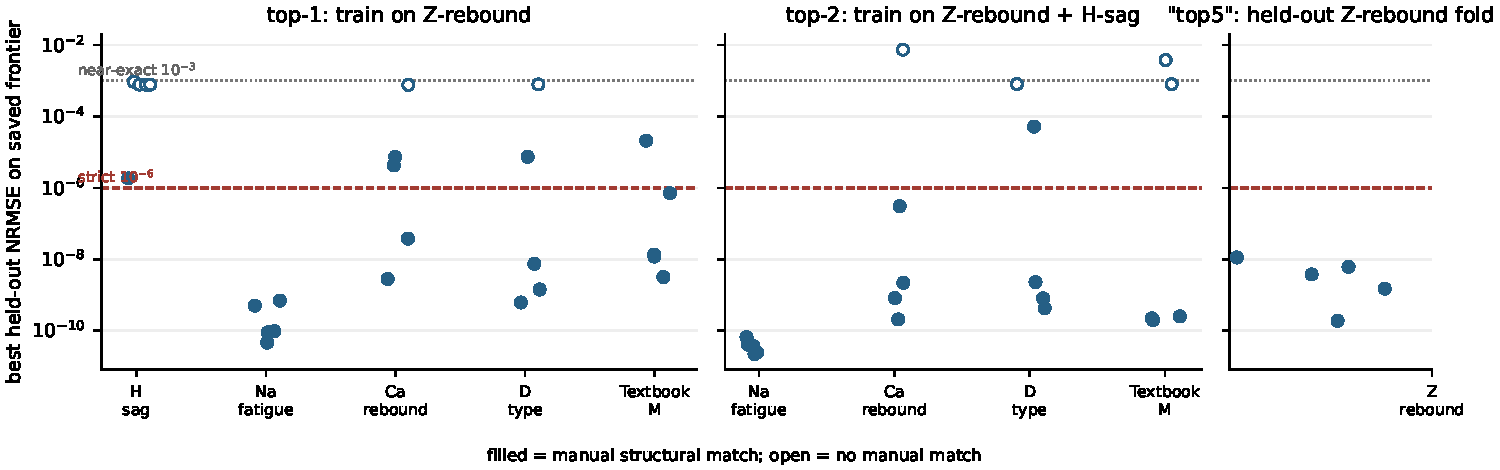
\includegraphics[width=0.91\linewidth,height=0.66\textheight,keepaspectratio]{historical_transfer_nrmse.pdf}

  \vspace{0.06cm}
  \small
  \begin{tabular}{@{}lccccl@{}}
    \toprule
    Regime & Training worlds & Held-out worlds & Manual matches & Rate & Interpretation \\
    \midrule
    top-1 & 1 & 5 & 19/25 & 76\% & one evolved outcome \\
    top-2 & 2 & 4 & 16/20 & 80\% & one evolved outcome \\
    ``top5'' & 5 & 1 & 5/5 & 100\% & one completed LOOCV fold \\
    \bottomrule
  \end{tabular}
  \source{Primary results: \texttt{runs/313196/neuron\_full\_eval/neuron\_results.json}, \texttt{runs/313195/neuron\_full\_eval/neuron\_results.json}, \texttt{runs/312780/neuron\_results.json}; manual audit: \texttt{reports/neuron\_manual\_match\_comparison.json}.}
\end{frame}

% 8
\begin{frame}[t]{Newest run 708907: ``uninformative prompt,'' raw held-out results}
  \begin{columns}[T,onlytextwidth]
    \begin{column}{0.70\textwidth}
      \centering
      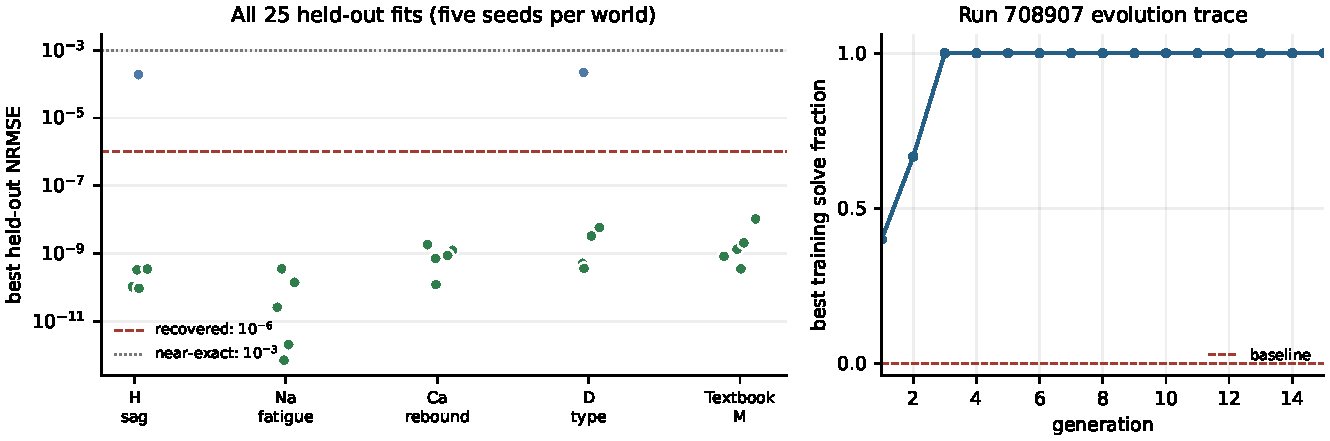
\includegraphics[width=\linewidth]{uninformative_raw_results.pdf}
    \end{column}
    \begin{column}{0.28\textwidth}
      \scriptsize
      \textbf{Prompt objective}

      ``Improve the algorithm's ability to discover the expression that generated the task data.''

      \vspace{0.08cm}
      \textbf{Training}
      \begin{itemize}
        \item Z-rebound only;
        \item baseline: 0/3 training solves;
        \item best bundle reaches 3/3 by generation 3.
      \end{itemize}

      \textbf{Held-out transfer}
      \begin{itemize}
        \item 23/25 recovered ($\le10^{-6}$);
        \item 2/25 near-exact ($\le10^{-3}$);
        \item no close or miss outcomes.
      \end{itemize}
    \end{column}
  \end{columns}

  \source{Primary artifacts: \texttt{runs/708907/run\_data.json}, \texttt{runs/708907/best\_bundles/best\_final.jl}, and \texttt{runs/708907/neuron\_full\_eval/neuron\_results.json}.}
\end{frame}

% 9
\begin{frame}[t]{A recovered equation matches the physical coefficients}
  \small
  Example: ``top5'' held-out Z-rebound, seed 10000, best frontier row. In physical units,
  \begin{align*}
  f_*(x)={}&x_0-120x_1x_2-36x_1x_3-4x_1x_4-0.3x_1\\
           &+6000x_2-2772x_3+480x_4-16.32.
  \end{align*}

  \begin{columns}[T,onlytextwidth]
    \begin{column}{0.62\textwidth}
      \centering
      \scriptsize
      \begin{tabular}{@{}lrrr@{}}
        \toprule
        Monomial & truth & discovered & absolute error \\
        \midrule
        $x_0=I_{\rm ext}$ & $1$ & $1.000000002$ & $2.1\times10^{-9}$ \\
        $V\phina$ & $-120$ & $-120.000000192$ & $1.9\times10^{-7}$ \\
        $\phina$ & $6000$ & $5999.999975$ & $2.5\times10^{-5}$ \\
        $V\phik$ & $-36$ & $-36.000000140$ & $1.4\times10^{-7}$ \\
        $\phik$ & $-2772$ & $-2772.000019$ & $1.9\times10^{-5}$ \\
        $V\phiz$ & $-4$ & $-3.999999978$ & $2.2\times10^{-8}$ \\
        $\phiz$ & $480$ & $479.999995$ & $5.1\times10^{-6}$ \\
        $V$ & $-0.3$ & $-0.299999829$ & $1.7\times10^{-7}$ \\
        $1$ & $-16.32$ & $-16.319975$ & $2.5\times10^{-5}$ \\
        \bottomrule
      \end{tabular}
    \end{column}
    \begin{column}{0.35\textwidth}
      \begin{block}{Numerical and structural checks}
        \begin{itemize}
          \item held-out $\nrmse=1.52\times10^{-9}$;
          \item all nine ground-truth monomials are present;
          \item no additional monomials;
          \item maximum absolute coefficient error $2.5\times10^{-5}$.
        \end{itemize}
      \end{block}
    \end{column}
  \end{columns}
  \source{Primary coefficient expansion: \texttt{reports/neuron\_top5\_symbolic\_recovery\_analysis.json}, recovery 0; source frontier: \texttt{runs/312780/neuron\_results.json}.}
\end{frame}

% 10
\begin{frame}[t]{Interpretation and remaining evidence gaps}
  \small
  \begin{columns}[T,onlytextwidth]
    \begin{column}{0.48\textwidth}
      \textbf{What the current evidence supports}
      \begin{itemize}
        \item PySR can recover the complete physical current-balance polynomial, not only a low-error surrogate.
        \item Bundles evolved on subsets of neuron mechanisms transfer to held-out worlds.
        \item Residual-guided additive mutation appears independently in the best top-1, top-2, top5, and uninformative-prompt bundles.
        \item Run 708907 shows that this motif does not require neuron-specific objective wording.
      \end{itemize}
    \end{column}
    \begin{column}{0.48\textwidth}
      \textbf{What remains to establish}
      \begin{itemize}
        \item Replicate meta-evolution runs before interpreting top-1/top-2/top5 as a learning curve.
        \item Complete the other five top5 leave-one-world-out folds.
        \item Apply the same physical-support manual audit to run 708907.
        \item Test whether residual-projection mutation transfers beyond this additive current-balance domain.
      \end{itemize}
    \end{column}
  \end{columns}

  \vspace{0.12cm}
  \begin{block}{Working conclusion}
    \scriptsize Meta-evolution repeatedly discovers a residual-fitting mutation that is structurally aligned with additive mechanistic laws.
  \end{block}
  \source{Interpretation based on the primary run artifacts cited throughout; metric distinctions and audit caveats are documented in \texttt{reports/neuron\_topk\_manual\_transfer\_report.pdf}.}
\end{frame}

\end{document}
